%\documentclass[letterpaper,10pt, jcp, aps]{revtex4-1}
\documentclass[superscriptaddress,pre,reprint,showpacs,onecolumn]{revtex4-1}

\usepackage[utf8]{inputenc}
\usepackage{amsmath, amsfonts}
\usepackage{graphicx}
\usepackage{natbib}
\usepackage{caption}
\usepackage{subcaption}
%\usepackage{authblk} parece ser que ya esta metido cuando usas preprint

\usepackage{hyperref}


%\bibliographystyle{alpha}

%opening

%\author{Rosa Rodríguez \& David P.~Sanders \& W. P. K. Zapfe}
%\affil{Departamento de Física, Facultad de Ciencias, Universidad Nacional Autónoma de México, Ciudad Universitaria, Del.~Coyoacán, México D.F. 04510, Mexico}

\usepackage{mathptmx}
% I dont know if that package is compatible with revtex.

\newcommand{\defeq}{:=}
\newcommand{\mean}[1]{\left \langle #1 \right \rangle}
\newcommand{\rd}[1]{\mathrm{d}{#1} \,}
\newcommand{\RR}{\mathbb{R}}
\newcommand{\vv}{\mathbf{v}}
\newcommand{\indicatorsymbol}{\mathbf{1}}
\newcommand{\indicator}[1]{\indicatorsymbol_{ \{   #1 \} } } 
\newcommand{\etal}{et al.\ } 

\setlength{\parskip}{10pt}
\setlength{\parindent}{0pt}


\begin{document}

\title{Exact hopping and collision times for two hard discs in a box}

\author{Rosa Rodríguez}
\email{rosa.g.asor@gmail.com }
\affiliation{Physics Department, McGill University}

\author{David P.~Sanders}
\email{dpsanders@ciencias.unam.mx}
\affiliation{Departamento de Física, Facultad de Ciencias, Universidad Nacional Autónoma de México, Ciudad Universitaria, Ciudad de México 04510, Mexico}

\author{W.~P.~Karel Zapfe}
\email{karelz@cinvestav.mx}
\affiliation{Departamento de Física, Facultad de Ciencias, Universidad Nacional Autónoma de México, Ciudad Universitaria, Ciudad de México 04510, Mexico}

\affiliation{CINVESTAV-IPN, Mexico}


\begin{abstract}
We study the molecular dynamics of two discs undergoing hard collisions in a rectangular box ("inertial dynamics").
Using the mapping to a billiard model, and results from ergodic theory, we obtain exact expressions for mean times between ``hops'' (horizontal or vertical interchanges), wall collisions and disc collisions, by calculating
volumes and cross-sectional areas in the four-dimensional configuration space.
In all cases, we compare exact analytical results against Monte Carlo simulations.
\end{abstract}

\maketitle



\section{Introduction}

%\typeout{`` this is ``  \the\columnwidth }

Collision times play a fundamental role in statistical mechanics, since properties
such as mixing, reaction and diffusion rates depend on them \cite{Boltz72, Tolman, VanKampen}.
A paradigmatic model, introduced by Boltzmann allmost 150 years ago \cite{Boltz72, SzaszBook00},
consists of a fluid of hard spheres colliding with each other, either in a periodic torus or 
a rectangular box.

The simplest such system, which is still non-trivial, is that of two discs in a box.
The discs move rectilinearly until they undergo
elastic collisions either with a wall of the box, or with one another; this has been called ``inertial motion'' (to distinguish it from Brownian motion) \cite{Bowles04}.
Phenomena such as transport, collision and reaction
have been studied in this systems, both analytically 
 \cite{Awazu01, Munakata02, Suh05} and numerically \cite{MacElroy2005}
 Events of physical interest in this system are \emph{hopping},
in which two particles interchange position, either vertically or horizontally,
\emph{collision} of the particles, with the box or with each other.
These have been studied numerically, for example in \cite{MacElroy2004}
 
Previous work
by Bowles \etal gives general quantitative results for the mean hopping 
time for both inertial and Brownian dynamics \cite{Bowles04}. THIS IS A DIFFERENT DEFINITION OF HOPPING TIME -- FIRST PASSAGE TIME.
They use arguments from Transition State Theory 
to provide expressions for the general behavior of these quantities, as functions of the
radius of the discs. %Their results show the adequate algebraic behavior.
A great deal of work has expanded along that line  \cite{Suh05, Ball09}.
There is also a statistical thermodynamic treatment by Munakata \etal 
which deals very comprehensively with partition functions, pressure,
and temperatures \cite{Munakata02, Munakata06}. 


In this paper, we obtain \emph{exact} analytical expressions for mean inter-hop and inter-collision times of two discs under 
inertial motion, as a function of the geometrical parameters of the system. Such a treatment is possible
 since the dynamics of $N$ hard discs in $d$ spatial dimensions
 is equivalent to a \emph{billiard model} in the $Nd$-dimensional configuration space, i.e. a \emph{single} point particle colliding elastically 
with suitable objects (``scatterers'') \cite{SzaszBook00}. 
In particular, the system of two discs in a box is hyperbolic and ergodic when the discs are able to pass each other \cite{Sim99}. 

We can thus apply a key result from ergodic theory on mean collision times \cite{Chernov97}, and hence obtain analytic expressions 
for times between hops, between wall collisions, and between disc collisions. These are also verified numerically. 
%The difficulty in the calculations lies in correctly accounting for various
%factors occurring in the expressions. 
In certain asymptotic regimes, we recover previously obtained power-law exponents \cite{Bowles04}.


%The previous  results on
%inertial dynamics can be extended  by particularizing 
%exact expressions for the mean return times (MRT). 
%We shall  obtain them through application of 
%Machta and Zwanzig formula for residence times \cite{MachtaZwan} ??
%We shall also  compare \emph{mean event times} with 
%\emph{mean first event times} (MFET),
%and give some arguments to explain the agreement between the two. 
%Brownian dynamics shall be discussed elsewhere \cite{WorkInProgress}.
%We shall also provide this paper with supplementary material 
%detailing the calculations. 



\section{Model: Two hard discs in a rectangular box}

We consider two hard discs with the same radius $r$,
in a box of width $w$ and height $h$; see Fig.~\ref{billar01}. 
The discs move inertially in the absence of forces, 
following straight line trajectories,
and undergo elastic collisions with each 
other and with the walls of the box.

\begin{figure}[h]
  \begin{center}
  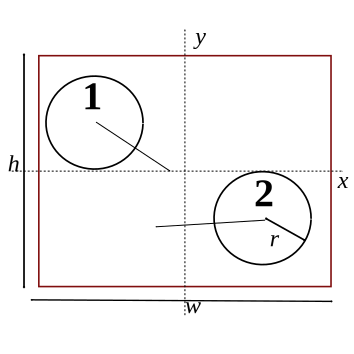
\includegraphics[width=0.40\textwidth]{figures/DiscosenCajaCuadrada01.pdf}
  \end{center}
  \caption{The billiard and its parameters. Coordinates
    have their origin at the geometrical center of the 
    billiard table.}\label{billar01}
\end{figure}


We denote the position of the center of the $i$th disc by 
$\mathbf{x}_i = (x_i, y_i)$, and its velocity by $\mathbf{v}_i = (u_i, v_i)$ for $i=1,2$. Since the discs are hard, 
their centers are restricted to the region 
$(x_i, y_i) \in [-a,a] \times [-b, b]$, where 
$a \defeq a(r) \defeq \frac{w}{2} - r $ and
$b \defeq b(r) \defeq \frac{h}{2} - r $.

The exclusion condition preventing the discs from overlapping is $(x_1-x_2)^2 + (y_1-y_2)^2 \ge (2r)^2$.
It is thus useful to perform an orthogonal transformation (rotation) to the following new coordinates:
\begin{equation}\label{cambiocoor01}
 x \defeq \frac{x_1 - x_2}{\sqrt{2}}; 
\quad X \defeq \frac{x_1 + x_2}{\sqrt{2}}; 
\quad y \defeq \frac{y_1 - y_2}{\sqrt{2}}; 
\quad Y \defeq \frac{y_1 + y_2}{\sqrt{2}}.
\end{equation}

%%This is WRONG, or better, is not precise enough.
In these coordinates, the configuration space is given by the following
intervals:
$x \in [-a \sqrt{2}, +a \sqrt{2}]$ with 
$X \in [-a \sqrt{2} + |x|, a \sqrt{2} - |x|]$; and 
 $y \in [-b \sqrt{2}, b \sqrt{2}]$ with $Y \in [-b \sqrt{2} + |y|, +b \sqrt{2} - |y|]$.
The non-overlapping constraint becomes $x^2 + y^2 \ge 2 r^2$.
The horizontal and vertical coordinates transform independently
from each other, and the Jacobian is in each case equal to $1$.

These constraints define a four-dimensional
rectangular prism, in which is embedded an excluded cylinder with a three-dimensional surface
(codimension 1).
This cylinder has radius $r\sqrt{2}$ and lies
in  a diagonal position along the axes $X, Y$.
The prism surface is the outer boundary of the configuration space,
while the cylinder is the excluded volume, and its surface
acts as a reflecting inner boundary.
The dynamics of the two discs is equivalent to a billiard model in this space, in which 
a point particle undergoes free flight until
encounter with a wall, then elastic reflection.
The outer borders are flat, so the
hyperbolicity is due to the inner dispersing
boundary \cite{Sim99}, which represents the collision of
two discs in the original space.


We take the mass of each disk as $m=1$, so that the kinetic energy
is $\frac{1}{2}(\mathbf{v}_1^2 + \mathbf{v}_2^2)$. We restrict attention to the energy surface with
$E = \frac{1}{2}$, so that the disc velocities satisfy $\mathbf{v}_1^2 + \mathbf{v}_2^2 = 1$.
Other values of the mass or energy correspond to a simple rescaling of the dynamics, with velocities differing
by a factor of
$\sqrt{2E/m}$, and corresponding factors in the times to be determined below.


\section{Mean collision time for billiard models}

\label{knownfacts}
%\subsection{Known facts on collision rates}

A system of $N$ hard spheres confined by hard walls in a $d$-dimensional
space may be treated as a billiard system 
in which a single point  particle undergoes free motion between reflecting obstacles 
in a $ (d N) $-dimensional configuration space \cite{Sinai70, Sim99, MarkChern}. 
%If the resulting billiard is ergodic and hyperbolic, then we know that
%these systems are equivalent to Bernoulli flows \cite{Gallavotti74}.
This can be thought of as a mean return time to the $(d-1)$-dimensional 
(i.e. co-dimension $1$) cross-section given by the wall boundaries.

For a particle with unit velocity moving in a general billiard table, there is 
an exact expression for the mean time between 
collisions of the particle with a given wall \cite{Chernov97}:

\begin{equation}\label{meanfreetime}
 \mean{\tau} = \frac{|Q|}{|A|s} \frac{|S^{d-1}|} {|B^{d-1}|}.
\end{equation}

\pmb{TODO: Check if the s is well explained on the text below.}

Here, $|Q|$ denotes the $d$-dimensional volume of the available 
space in the billiard and 
$|A|$ the $(d-1)$-dimensional area of the cross-section.
 $|S^{d-1}|$ is the $(d-1)$-dimensional area of the unit sphere in $\RR^d$, given by
\begin{equation}
  |S^{d-1}| = \frac{2 \pi^{d/2}}{\Gamma(d/2)},
\end{equation}
where $\Gamma(\cdot)$ is the gamma function. 
$|B^{d-1}|$ is the volume of the unit ball 
in $\RR^{d-1}$, given by $|B^{d-1}| = |S^{d-2}| / (d-1)$.
Machta and Zwanzig \cite{MachtaZwan} used a similar method to derive an escape 
time across a virtual boundary by treating it as a recurrence time.
%Since it is an escape time, they used velocities whose components point only 
%perpendicularly to the ``exit wall''.

In our case, we are interested in the mean return time to 
several types of co-dimension-$1$ cross section.
The first, giving the ``hopping time'', 
is defined by the moment
in which the discs interchange their horizontal or vertical position, i.e.
\begin{equation} \label{condchoque}
x_1 = x_2  \qquad \text{or} \qquad y_1 = y_2.
\end{equation}
In this kind of events, the cross-section can be reached from either side, so that the area
$A$ is effectively twice as large; this will be given by a ``sidedness'' factor $s = 1$ or $s=2$ in the formula
for $\mean{\tau}$.

The other events of interest are collisions of disc number 1 with the right wall, and mutual
collisions between discs 1 and 2.
%
%Given that each disk has different momentum, but
%they can interchange it without affecting the
%total energy, we take into account the mass $m$ of each disk 
%and the total kinetic energy $E$.
%If both discs have the same mass then $\sum_i \vv_i^2 = 2E / m$.
%The above result, as derived by Chernov, 
%was for the case $\sum_i \vv_i^2 = 1$, or $m=1$ and $E=\frac{1}{2}$.  
%For more general values of $E$ and $m$, 
%we are simply working on a different energy surface in phase space. 
%The particle trajectories are identical but the velocities differ
%by a factor of
%$\sqrt{2E/m}$. All times must divided by this value, 
%giving for
%the mean time between events the general formula:
%\begin{equation} \label{meantimegeneral}
%  \mean{\tau} =  \frac{1}{\sqrt{2E / m}} 
%\frac{|Q| \, |S^3|} {s \, |A| \, |B^3|},	
%\end{equation}
%where $s$ is $1$ or $2$ depending if the cross section can be reached
%in one or two sides.

%We respect the convention of $E=1/2, m=1$ and we end up with
%\begin{equation} \label{meantimegeneralredux}
%   \frac{1}{\sqrt{2E / m}} 
%   \frac{|S^3|}{|B^3|}=\frac{3\pi}{2}.	 
%\end{equation}

To calculate the mean times of interest, it is thus necessary to calculate
the 4-dimensional volume $V$ of the available space, and the cross-sectional area $A$ 
for each type of event of interest. The main difficulty consists of correctly accounting for multiplicative factors associated to the different 
types of areas.
%
%
%The next step is obtaining the Volume (4 dimensional measure) of
%the available space and the Area (3 dimensional induced measure) of
%the collision conditions. We devote the next section to
%show the procedure, details can be found in the Appendix.


\section{Calculation of volume and areas}

%The configuration
%space is an four dimensional prism with a four dimensional
%cylinder subtracted.
%The calculation can be carried out indirectly,
% using indicator functions for the
%available space or for the prohibited space.

\subsection{Volume of available space}


We denote by $Z := \{ \mathbf{x} \in \mathbb{R}^4: (x_1-x_2)^2 + (y_1-y_2)^2 \ge (2r)^2 \}$ 
the complement of the cylinder in the configuration space.
The four-dimensional available volume $V_\text{free}$ is then given by
\begin{align}\label{volindic}
V_\text{free} &= 
\int_{x_1 = -a}^a  \int_{x_2 = -a}^a  \int_{y_1 = -b}^b \int_{y_2 = -b}^b
 \, \indicator{ (x_1-x_2)^2 + (y_1-y_2)^2 \ge (2r)^2 } \,
\rd x_1 \rd x_2 \rd y_1 \rd y_2 \\
&=
\int \indicatorsymbol_Z(\mathbf{x}) \, \mathrm{d} \mathbf{x},
\end{align}
where
$$ \int  \mathrm{d} \mathbf{x} :=  \int_{x_1 = -a}^a  \int_{x_2 = -a}^a  \int_{y_1 = -b}^b \int_{y_2 = -b}^b$$
is a four-dimensional integral over the whole volume, and 
$\indicatorsymbol_Z$ is the indicator function of the set $Z$, 
given by $\indicatorsymbol_Z (\mathbf{x}) = 1$ if $\mathbf{x} \in Z$, and $=0$ if $\mathbf{x} \notin Z$.
Fig.~\ref{diagintegral01} shows a diagram of the product of
spaces that give origin to the configuration space.
Recall that $a$ and $b$ are functions of $r$, 
but we suppress this explicit dependence for simplicity.

\begin{figure}[h]
  \begin{center}
    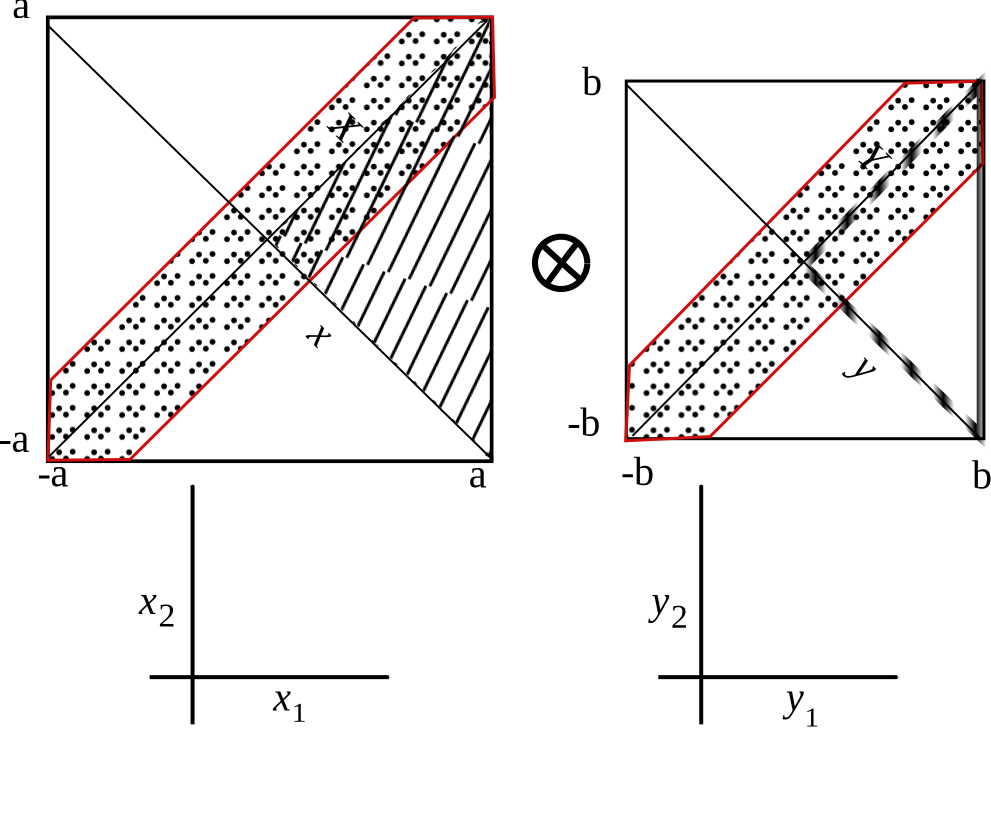
\includegraphics[width=0.45\textwidth]{figures/diagramintegra01.pdf}
  \end{center}
  \caption{The space to integrate is the product of the spaces
    belonging to horizontal and vertical coordinates. The dotted
    bands show the excluded set, that is, the complement of $Z$, where the condition 
    $ (x_1-x_2)^2 + (y_1-y_2)^2 \ge (2r)^2 $ is not satisfied.
    The width of each band is dependent on the particular 
    point of evaluation
    on the other subspace. Due to 
    symmetry, we only evaluate the hatched area and
    multiply the result by 16. I DON'T UNDERSTAND THIS PICTURE.
    \pmb{I do not know if I can make it simpler or give a sequence
    of pictures so that is more understandable}
    \label{diagintegral01}  
    }
\end{figure}

It is easiest to represent the  
excluded cylinder in the coordinates defined in 
Eq.~\ref{cambiocoor01}, since the coordinates $X$ and $Y$ 
do not appear in the exclusion condition:
\begin{equation}\label{integraltotal}
 V_\text{free} = \\ \int\limits_{x=-a \sqrt{2}}^{a \sqrt{2}} \rd x 
\int\limits_{X=-a \sqrt{2} + |x| }^{a \sqrt{2} - |x|}  \rd X
 \int\limits_{y=-b \sqrt{2}}^{b \sqrt{2}} \rd y
\int\limits_{Y=-b \sqrt{2} + |y| }^{b \sqrt{2}-|y|}  \rd Y
\, \indicator{ x^2 + y^2 \ge 2r^2  }.
\end{equation}
Since $X$ and $Y$ do not appear in the integrand, those integrals are trivial, giving
\begin{align}
 V_\text{free}  &= \int\limits_{x=-a \sqrt{2}}^{a \sqrt{2}} \rd x  \int\limits_{y=-b \sqrt{2}}^{b \sqrt{2}} \rd y
2 \left( a \sqrt{2} - |x| \right) \, 2 \left( b \sqrt{2} - |y| \right) \indicator{ x^2 + y^2 \ge 2r^2 } \\
 &= 16 \int\limits_{x=0}^{a \sqrt{2}} \rd x  \int\limits_{y=0}^{b \sqrt{2}} \rd y 
\left( a \sqrt{2} - x \right) \left( b \sqrt{2} - y \right) \indicator{ x^2 + y^2 \ge 2r^2 },
\end{align}
where we have used symmetry to reduce to one octant.
Thus $V_\text{free} = 16(I_1 + I_2)$, where $I_1$ is the region where the value of $y$
is affected by the exclusion condition and $I_2$ is where it is not affected
by it.  FIG?
We have
\begin{align}
 I_1 &= \int\limits_{x=0}^{r\sqrt{2}} \rd x \int\limits_{y = \sqrt{ 2r^2 - x^2}}^{b \sqrt{2}} \rd y
\left( b \sqrt{2} - y \right)  \left( a \sqrt{2} - x \right) \\
&= 	
2 a b^{2} r  + \textstyle \frac{1}{6} (a+b) (2r)^{3} - \frac{1}{32}  (2r)^{4} - \frac{1}{4} {\left(\pi a b + b^{2}\right)} (2r)^2,
\end{align}
and
\begin{align}
 I_2 &= \int\limits_{x=r  \sqrt{2}}^{a \sqrt{2}} \rd x  \int\limits_{y = 0}^{b \sqrt{2}} \rd y
 \left( b \sqrt{2} - y \right)  \left( a \sqrt{2} - x \right)  \\
&=	
{\left( a^{2} - 2ar +   r^{2}\right)} b^{2}.
\end{align}
Thus 
\begin{align}\label{volumeabd}
 V_\text{free}
 & =  16 a^{2} b^{2}  - 16 \pi a b r^{2} + \textstyle \frac{64}{3} (a+b) r^{3}  - 8 r^{4} \\
&= V_\text{prism} - V_\text{cyl},
\end{align}
as previously obtained by Munakata and Hu \cite{Munakata02}.
It is useful to split this expression into the total volume of the prism 
$V_\text{prism}=16 a^2 b^2$, and the cylindrical volume excluded by the overlapping
condition, 
$V_\text{cyl}=  16 \pi a b r^{2} - \textstyle \frac{64}{3} (a+b) r^{3}  + 8 r^{4}$.

The substitutions $a\rightarrow (w-2r)/2$ and $b\rightarrow (h-2r)/2$ give us
 the volume as a function of the radius, for fixed table size:
\begin{equation}\label{volumewhd}
 V_\text{free} 
= (w-2r)^{2} (h-2r)^{2}  - 
 \pi (w-2r)(h-2r) 4 r^{2} + 
\textstyle \frac{32}{3} (w+h-2r) r^{3}  
- 8^{4}.
\end{equation}

Note that the above formula is correct only when both
vertical and horizontal hopping are possible, i.e., when $h > 4r$ and $w > 4r$.
When either or both is no longer possible, the 
integration limits for $X$ and $Y$ in \eqref{integraltotal} are altered; 
see Appendix ~\ref{app:area_volume} for the corresponding results.

As an example, we consider the case where vertical hopping is possible
and horizontal is excluded,  $w \geq h$.
This case is divided into two sub-cases: if
$ h \leq  w < 2 h $ there is a value for $r$ for which hopping is not possible,
but the discs still fit inside. For $ 2 h \leq w $, vertical hopping is
possible until $ 2 r= h$ (where vertical movement is impossible). These cases
can be thought of as the configuration space becoming disjoint, and
some of the cross section areas staying outside it. Thanks to the symmetry of
the problem, in many cases the cross-section areas and 
volumes become disjoint components sharing the same fraction of
the total volume, making the transition smooth.

We cite the  result for $h/4  <r< w/4$ for illustrative purposes.
For readability we define another auxiliary variable,
$c=\sqrt{4r^2-b^2}$:
\begin{multline}\label{VolumenCasoFeo}
V_{h/4<r<w/4} = 32abr^2[\arccos(b/2r)-\arccos(a/2r))]\\
+\frac{64 r^3}{3 }[a((b-a)/2r)-b(c/2r+\sqrt{4r^2-a^2}/2r)]\\
-2r^2 (b^2-a^2)\\ 
+16[ a b^2 c (4\sqrt{2}-1-\sqrt{2}/3)
+c^2b^2 (\sqrt{2}/3-1) \big]
\end{multline}
In the case that $r$ is larger than both $h/4, w/4$, one must take
into account a similar
contribution which inverts the roles of $a$ and $b$. Then there is
a case where hopping is impossible. 

In order to not to pick a degenerate case for our numerical simulations,
we have set $w=1.5, h=1$. This covers all of the uses of the general volume formulas.


We have checked this result with standard rejection sampling Monte Carlo simulations, 
by generating uniform random positions for the disc centers in 
$[-a,a] \times [-b,b]$ and 
counting the fraction of initial conditions for 
which the two discs do not overlap (rejecting those where is overlap); the results are shown in Fig.~\ref{VolMonteC}.



\begin{figure}[h]
\centering
\includegraphics[width=0.45\textwidth]{./figures/FreeVolume01.png}
\caption{Free avaible Volume in configuration space as function of radius. The
  line labeled $rhmax$ is the limit for horizontal hopping, and the one labeled
  $rvmax$ is the limit for vertical hopping. The transition between formulas
is continous, as it should be.}\label{VolMonteC}%% 
\end{figure}


The following subsections shall only show the formulas for $r<w/4, h/4$.
Bear in mind that some of the dynamics are possible above this limit,
it is only the position interchange that gets excluded. \\




\subsection{Cross section areas}\label{areahop}

The areas of cross sections $A$ are surface areas of 3-dimensional surfaces (manifolds) $S$ embedded in the configuration space,
defined by algebraic equations of the form $g(\mathbf{x}) = 0$, so that $S = g^{-1}(0)$ is the zero set of $g$.
The surface area of $S$ is then given by
\begin{equation}
A(S) = \int \indicatorsymbol_Z(\mathbf{x}) \, \delta(g(\mathbf{x})) \, \mathrm{d} \mathbf{x}.
\label{eq:surface-area}
\end{equation}
To evaluate this, we use the relation in H\"ormanders Book, sec 6.1 \cite{Hormander83}:
\begin{equation}
\int_{\mathbf{R}^d} f(\mathbf{x}) \, \delta(g(\mathbf{x})) \, \mathrm{d} \mathbf{x} = \int_{g^{-1}(0)}\frac{f(\mathbf{x})}{\| \mathbf{\nabla}g(\mathbf{x}) \|} \, \mathrm{d}S,
\label{eq:surface-dirac}
\end{equation}
where the integral on the right-hand side is over the surface $g^{-1}(0)$.

The appearance of the normalization factor $\| \mathbf{\nabla}g(\mathbf{x}) \|$ can be understood intuitively by considering how to verify numerically these surface areas. One possible technique is to use rejection sampling to sample the volume given by $|g(\mathbf{x})| \le \eta$ for some $\eta$.

The efficiency could be improved by a Markov Chain Monte Carlo algorithm that rejects steps that take the dynamics outside the set of interest.

\subsubsection{Hopping}

\pmb{Checa bien esto: esta es la discucion infinita que hemos tenido mil veces.}
The condition for vertical hopping is when the vertical positions of the two discs are equal FIG, that is: $y_1-y_2=0$. Nevertheless, this doesn't represent the area for hopping,
in the same way that $y=x$ and making $ \int \delta(y-x) dx dy$  would give you an erroneus length of the diagonal line. The expression that gives the area is
$$g_\text{hop}(\mathbf{x}) := (y_1 - y_2)/\sqrt{2} = 0.$$
Applying Eqs.~\eqref{eq:surface-area} and \eqref{eq:surface-dirac}, we obtain
%
\begin{widetext}
\begin{equation}
 A_\text{hop} = \int\limits_{x_1 = -a}^a \rd x_1 \int\limits_{x_2 = -a}^a \rd x_2 
\int\limits_{y_1 = -b}^b \rd y_1 \int\limits_{y_2 = -b}^b \rd y_2 \, \indicator{ (x_1-x_2)^2 + (y_1-y_2)^2 \ge (2r)^2 } \, \delta(\frac{y_1-y_2}{\sqrt{2}}).
\end{equation}
\end{widetext}
IS THIS WRITTEN CORRECTLY?
\pmb{NOW IT IS}

Carrying out the integrals gives
 \begin{equation}\label{AreaH}
 A_\text{hop}  =  16 \sqrt{2} b(a-r)^2.
\end{equation}
As before, the formula is no longer valid for $r > w/4$. In this case,
vertical hopping becomes impossible for a larger radius.

Monte Carlo simulations to calculate this area must also be done carefully.
See Appendix: Calculate distance to surface.


In this case we 
by counted the proportion of successful placements of hard discs 
for which the distance 
$|y_1 - y_2|$ was within a small tolerance of $0$. 
Results are shown in figure \ref{AreaHopp01}.

\begin{figure}[h]
\centering
\includegraphics[width=0.45\textwidth]{./figures/AreaHop01.png}
\caption{The hopping area, $A_\text{hop}$, 
  indicated in the formula in eq. \ref{AreaH}. As explained
in the text, it gives nonsense for $r>1/4$, but numerical values stay
exactly at zero, the correct value. } 
\label{AreaHopp01}
\end{figure}


\subsubsection{Disc collisions}

The area which represents collisions between the two discs is the surface area of the cylinder
that lies within the prism, given by
$$g_\text{collision}(\mathbf{x}) := ((x_1-x_2)/\sqrt{2})^2 + ((y_1-y_2)/\sqrt{2})^2
- 2*(r)^2) = 0.$$
The factors have the same reasons to appear as in the case of the hop condition.

For $r<w/4$, we find for the corresponding area
\begin{align}\label{AreaChoque}
A_\text{collision} & =  \sqrt{2} (
16\pi a b r -32 (a+b)r^2 +16 r^3).
\end{align}

We proceed in the same manner as last section, checking numerically which
random
conditions fall at a small tolerance of $0$ from the collision condition, and
plotting this as a fraction of the total volume. The result is shown in the
figure \ref{AreaChoqueTeoyNum}. 
\begin{figure}
\centering
\includegraphics[width=0.45\textwidth]{./figures/AreaCol01.png}
\caption{The numerical and theoretical calculation for the Area of the cross section
for collision between the discs.  The theoretical formula 
\ref{AreaChoque} breaks down at
$r>1/4$, but we have here used the general formula.}
\label{AreaChoqueTeoyNum}.
\end{figure}


\subsubsection{Wall collisions}

We restrict attention to collisions of disc $1$ with the right wall, for which
$$g_\text{wall}(\mathbf{x}) = x_1 - a = 0.$$
The corresponding area, after taking account of the delta, is
\begin{equation}\label{areaindic}
 A_\mathrm{wall} =  \int_{x_2 = -a}^a \rd x_2 
\int_{y_1 = -b}^b \rd y_1 \int_{y_2 = -b}^b \rd y_2 \, \indicator{ (a-x_2)^2 + (y_1-y_2)^2 \ge 4 r^2 }
\end{equation}
The integration gives
\begin{align}\label{areax1p}
 A_\mathrm{wall} & = 8 a b^2-4  \pi b r^2 +\frac{16}{3}r^3 .
 % & = 2(w-d)^2 (h-2)^2- \frac{\pi}{2} (h-d) d^2 +\frac{2}{3}d^3 
\end{align}
Once again, a simple Monte Carlo procedure verifies this result,
shown in Fig.~\ref{area1derecha}.
This time, the correcting factors of $\sqrt{2}$ don't appear, as
these geometrical areas are orthogonal or parallel to the original
position coordinates.


\begin{figure}
\centering
\includegraphics[width=0.45\textwidth]{./figures/AreaWall01.png}
\caption{The numerical and theoretical calculation for the cross section area
for the impact of a determined disk with the right wall, as in eq. \ref{areaindic}.
Again, the general formula has been used.}
\label{area1derecha}.
\end{figure}

Taking into account the symmetry of the expression for either disc
 bouncing on either of the vertical walls, the
cross section area for this event is four times $A_\textrm{wall}$. For horizontal wall 
collisions, the roles of $a$ and $b$ are switched.
Thus the cross section area for any impact on any wall is
\begin{align}\label{areawalls}
 A_\text{walls} & = 32 a b (a+b)-16 \pi r^2 (a+b) +\frac{128}{3}r^3.
 %&=  4 (w-d) (h-d)  (w+h-2d) -2 \pi d^2 (w + h-2 d) +\frac{16}{3}d^3. 
\end{align}
%The cross section area for any collision is then 
%the sum of the last expression
%and the area for collisions between discs, \eqref{AreaChoque}.


\section{Exact mean event times}

In this section, we apply the results of the last section to give
exact mean inter-hop times, as well as wall collision and disc collision times.

%The three formulas have been checadas entre ellas y con gnuplot
% y la numerica: no aparecen factores espurios de raiz de dos
\subsection{Mean hopping time}

 CHECK THE FORMULAS AND REVISIT THE ASYMPTOTICS 
\pmb{Done}
 
Inserting the results of the previous section 
into the formula for the mean times for crossing
surfaces of section, \eqref{meantimegeneral}, finally gives exact mean inter-event times.

For vertical
hops we have:
\begin{equation}\label{hoptau}
 \mean{\tau_\text{hop}} = 	
\frac{3 \pi}{4\sqrt{2}}
\frac{2 a^{2} b^{2}  - 2 \pi a b r^{2} + \textstyle \frac{a+b}{3}  (2r)^{3}  -  r^4}
{ b \sqrt{2}  ( a - r )^2}.
\end{equation}
Recall that here there is a factor $s = 2$.
The limiting form for small discs is revealing: a constant
that depends only on the height of the table, since then the discs have almost no interaction:
\begin{equation}\label{hoptaulimit}
 \mean{\tau_\text{hop}} \overset{r \to 0}{\sim}
\frac{3 \pi}{8\sqrt{2}}h.
\end{equation}
Also of interest is the limit $r\sim w/4$, where vertical hopping becomes
impossible.  The lower term goes to zero quadratically, while the avaible volume
is still positive (except in the degenerate case that $w=2h$). The exact expression
is cumbersome, due to the fact that the general volume expression in such a
case is loaded with inverse trigonometric functions and doesn't appeal to
intuiton, but the leading term is exactly $w^2(h/2-w/4)^2$, so, it goes to infinity
like $1/x^2$. 



\subsection{Mean disc collision time}

For collisions between discs, we have, for the case $r<w/4$,
\begin{equation}\label{colltau}
 \mean{\tau_\text{coll}} = 	
\frac{3 \pi}{2\sqrt{2}}
\frac {2 a^{2} b^{2}  - 2 \pi a b r^{2} + \textstyle \frac{a+b}{3}  (2r)^{3}  -  r^4}
{2\pi a b r -4(a+b)r^2+2r^3}
\end{equation}
As expected, this goes to infinity with very small radius, its behaviour
approaching the expression
\begin{equation}\label{colltaulim0}
\mean{\tau_\text{coll}} \overset{r \to 0}{\sim}
\frac{3}{8\sqrt{2}}\frac{wh}{r}
\end{equation}
For the case in which the discs narrowly fit inside the table we need to
use the more cumbersome expression in eq. \ref{VolumenCasoFeo} and
the corresponding area. The time between collisions should go to zero.


\subsection{Mean wall collision time}

Lastly, for a specific disc colliding with a specific vertical wall we have
\begin{equation}\label{impactwall}
 \mean{\tau_\text{wall}} = 	
\frac{3 \pi}{2\sqrt{2}}
\frac { 2a^{2} b^{2}  -  2\pi a b r^{2} + \frac{a+b}{3}(2r)^3 - r^4}
{ab^2-\pi/2b r^2 + \frac{16}{3} r^3 },
\end{equation}
in the case that $r<h/4$. The limiting form for very small r is
quite interesting, as is only dependant on the width of the table and is exactly
$3\pi w/(2)$. In the numerics this appears as the intersection with the $\tau$
axis.

For the case that $r\approx h/4$ we would have two limiting forms,
as there is a discontinuity on the avaible Volume, but it is exactly
a factor of two discontinuity, so we can check from above and see
if it coincides. The expression is hardly appealing, as the Volume becomes
a fourth order polynomial of $h,w$ and the area a third order polinomial of
the same quantities. In our particular case this becomes,
after some juggling with the variables the approximate value 3.34. 


%Adding the areas representing the impact on the walls and
%the collisions on the discs, we  obtain
%the expression for \emph{any} 
%collision in the system:
%\begin{equation}\label{impactany}
% \mean{\tau_\text{any}} = 	
%\frac{3 \pi}{2\sqrt{2}}
%\frac { 2a^{2} b^{2}  -  2\pi a b r^{2} + \frac{a+b}{3}(2r)^3 - r^4}
%{4ab(a+b)+2 \pi \sqrt{2} abr-(2\pi+4\sqrt{2})(a+b)r^2+(\frac{16}{3}+2\sqrt{2})r^3}.
%\end{equation}

%In the limit $r\rightarrow 0$ this is asymptotic to $3 \pi (hw)/(8\sqrt{2}(h+w))$.
%This should correspond to the average impact time on the walls
%for non-interacting point particles.
%but, then, such as system would not be chaotic and the limit is senseless.
%On the other hand, for the limit of radius as large as possible, we shall
%again use the extended expressions in the formula for volume and area.


\subsection{Comparison with numerics}

In this section, we compare the analytical results obtained with direct numerical simulations of
event times.

%\subsection{Mean times for events}


The next three figures, \ref{MeanHopp01}, \ref{MeanCol01}, and \ref{MeanImp01},  
we compare the
numerical and analytically curves for the mean return times of different events.

\begin{figure}[h]
  \centering
  \includegraphics[width=0.45\textwidth]{./figures/VertHop01.png}
  \caption{The mean hopping time as function of the radius, Energy, mass, 
and geometry fixed, numeric and Analytic results.}\label{MeanHopp01}
\end{figure}

\begin{figure}[h]
  \centering
  \includegraphics[width=0.45\textwidth]{./figures/DiscCollitions01.png}
  \caption{The mean collision time as function of the radius. Same
    specifications as the last figure. }\label{MeanCol01}
\end{figure}


\begin{figure}[h]
  \centering
  \includegraphics[width=0.45\textwidth]{./figures/HitRightWall01.png}
  \caption{The mean impact-on-walls time as function of the radius. Again, same
    notes as the figure \ref{MeanHopp01}}\label{MeanImp01}.
\end{figure}

\pmb{Shall we plot the distributions for fixed interesting r? }

%\section{Mean first event times}
%
%Although we do not have a formula for the mean first event time as
%we have for the mean return times, we can, with a slight modification
%of our code, investigate the behaviour for these quantities. We have 
%an interesting result: most \emph{first event times} deviate very slightly,
%although systematically, from the \emph{mean return times}.
%
%%This could be explained as follows:
%%In an ergodic regime we could simply average over a sufficiently large
%%sample of initial conditions instead of following each trajectory
%%and sampling events along it. This means that the mean return time
%%coincides with the mean first return time for large enough samples.
%%A \emph{mean first event time} could be though of a \emph{mean
%%first return time} with erroneous initial conditions, as if the
%%trajectories had started, so there would be an \emph{average offset}
%%for the times. As we show numerically, this is indeed the case. 
%
%
%\begin{figure}[h]
%  \centering
%  \includegraphics[width=0.45\textwidth]{./FigurasPerfectas/FistHopTime01-ForPaper.pdf}
%  \caption{The mean first event time for the hopping event (MFET).
%    We compare against the \emph{mean return time} (MRT), theoretical
%and numerical. We observe how it is conterintuitivelly slightly longer,
%but the qualitative behaviour is almost equal. A logarithmic inset
%shows the behaviour across a wider range of scales. }\label{FirstHopp01}
%\end{figure}cd
%
%\begin{figure}[h]
%  \centering
%  \includegraphics[width=0.45\textwidth]{./FigurasPerfectas/FistCollTime02-ForPaper.pdf}
%  \caption{The mean first collision time as function of the radius.
%    Here we have  a slighter shorter time as the radius increases. The difference
%is more notorious on the semi-log plot in the inset. 
% }\label{FirstCol01}
%\end{figure}
%
%\begin{figure}[h]
%  \centering
%  \includegraphics[width=0.45\textwidth]{./FigurasPerfectas/FistImpactTime01-ForPaper.pdf}
%  \caption{The mean first impact-on-walls time as function of the radius. Again, 
%    we observe the same qualitative behaviour but now the whole range is below
%    the mean return time. This is to be expected, as for any initial condition
%    we would have a past condition on the wall. For very
%    large radius the step away from the wall is almost negligible.}\label{FirstImp01}.
%\end{figure}
%

\section{Conclusions}

We have calculated exact analytic expressions for mean hopping and
collision times in the paradigmatic model of two discs in a hard box
%The 
%results which have helped us to do this came from the
%extensive theory of chaotic billiards. The subjacent theory
%of ergodic systems already contains strong theorems and formulas
%that only need judiciously application to show their 
%elucidating power. The step done by Machta and Zwanzig in
%that direction is a clear example of grounding that
%theory in applicable research. We have expanded
%that line by showing that other phenomena can be modeled
%as return times to appropriately chosen surfaces of section. 
The analytical results derived 
confirm the limiting behaviour obtained
by Bowles \etal by a different method, and Monte Carlo simulations confirm 
the results. 

The results may be extended to different radii and to more spatial dimensions, albeit
with an increase in algebraic difficulty.

%Even though no exact expression is available for first event times, these follow
%the same qualitative behaviour as the mean return times.

%The same technique can be further exploited for some other
%qualities simply by solving the adequate measures
%of volumes and areas. For Transport and Reaction problems
%the results that we have shown here could be made to serve
%the purpose of deriving the corresponding constants from first
%principles.

REF: 3 discs

2 hard spheres in a spherical pore: conservation laws

\appendix
\section{Area and volume calculations}
\label{app:area_volume}

\subsection{Volume}\label{VolApen}

We use the same notation as in the rest of the paper.
Do simplify the formulas, we do not write explicitly the dependence of $a$ and $b$ on $r$.

An implicit assumption was made on the limits of integration in \eqref{integraltotal}. If $w, h > 4r$, then the limits of integration
are unaffected by the radius of the circles.
In order to avoid uninteresting constant terms
in the formulas, we integrate
the excluded volume, instead of the available one. 

We begin the derivation after integrating out $X$ and $Y$:
\begin{equation}\label{VolumenGeneral}
V/16 =\iint \rd x \rd y \left[ 2ab-\sqrt{2}(ay+bx)+x y \right]
\indicator{x^2+y^2 < 2r^2 }.
\end{equation}
A diagram helps us visualize the limits of integration. The most general
case is (without loss of generality) $h < w < 2h$, so that, as the radius of the
discs increases, we can pass from the regime where both vertical and horizontal
hopping occur, to the one where only vertical hopping
is possible, to the one where no hopping is possible but a certain amount of movement
can still occur. The three regimes are characterized by the following inequalities:
\begin{itemize}
\item All hopping possible: $0<r \leq h/4$
\item Only vertical hopping possible: $h/4 < r \leq w/4$
\item No hopping possible: $w/4 < r < (h+w-\sqrt{2hw})/2$
\end{itemize}
The largest possible radius is illustrated in Fig.~\ref{radiomaximo}.

\begin{figure}[h]
  \centering
  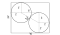
\includegraphics[width=0.4\textwidth]{figures/DiagramaRadioMaximo.pdf}
  \caption{The largest possible radius for $h<w<2h$. From the diagram
    one can see that $t^2+v^2=(2r)^2$, $h=t+2r$ and $w=v+2r$, from which
    one can deduce the value for $r$.}
  \label{radiomaximo}
\end{figure}

We shall look at these regimes on the integration space. The first one is solved
in the main text, but we shall repeat it here with a different coordinate system, so as to
make some points. In Fig.~\ref{diaglimites} we present the three regimes as
the shaded area where we perform the integration. 
  
\begin{figure}[h]
        \centering
        \begin{subfigure}[b]{0.32\textwidth}
          \centering
          \includegraphics[width=\textwidth]{figures/DiagramaIntegraCaso1.pdf}
          \caption{$r<b$}
          \label{Caso1}
        \end{subfigure}%
        ~ %add desired spacing between images, e. g. ~, \quad, \qquad etc.
        % (or a blank line to force the subfigure onto a new line)
        \begin{subfigure}[b]{0.32\textwidth}
          \centering
          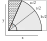
\includegraphics[width=\textwidth]{figures/DiagramaIntegraCaso2.pdf}
          \caption{$b<r<a$}
          \label{Caso2}
        \end{subfigure}%
        ~ %add desired spacing between images, e. g. ~, \quad, \qquad etc.
          %(or a blank line to force the subfigure onto a new line)
        \begin{subfigure}[b]{0.32\textwidth}
          \centering
          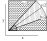
\includegraphics[width=\textwidth]{figures/DiagramaIntegraCaso3.pdf}
          \caption{$a,b<r$}
          \label{Caso3}
        \end{subfigure}%
        \caption{The three possible cases. The shaded area is where the integral
          must be evaluated. In the first case all hopping is possible, the middle case
          only allows for vertical hopping and the last case excludes hopping but there
        is still possibility for the discs to fit inside the table.}
\label{CasosIntegra}
\end{figure}
The shaded area in figure \ref{CasosIntegra} represents where the indicator function
has value 1. We can translate that to well chosen limits of integration. Notice
how the hatched area in the first three cases may be integrated in polar coordinates
simplifying the three cases to three cases of evaluation. We shall call the
indefinite integral $V_h(r,\alpha,\beta)$ (h is for ``hatched'').
As can be seen from figure \ref{CasosIntegra}, the all hopping possible regime
means that $\alpha = \pi/2, \beta=0$, the vertical hopping regime is where
$\alpha < \pi/2, \beta=0$, and the no hopping regime is where $\pi/2 > \alpha > \beta > 0$.

\begin{equation}\label{Vhatch1}
\begin{split}
V_h(r,\alpha,\beta)/16 &=
\iint \rd x \rd y \left[ 2ab-\sqrt{2}(ay+bx)+x y \right]
\indicator{x^2 + y^2 < 2r^2}\\
&=
\iint \rd \rho \rd \theta \rho 
\left[ 2ab -\sqrt{2}(a\rho\sin\theta+b\rho\cos\theta) +\rho^2 \cos\theta\sin\theta \right]
\indicator{\rho^2<2r^2 }
\end{split}
\end{equation}
The indicator function becomes the limits over the $\rho$ integrating variable.
We set the $\alpha, \beta$ as the other two limits. Then perform the
integral over the $\rho$ which doesn't change in the three regimes.
\begin{equation}
  \begin{split}
 V_h(r,\alpha,\beta)/16 &=\iint\limits_{\beta,0}^{\alpha,r\sqrt{2}} \rd \rho \rd \theta \rho (2ab
-\sqrt{2}(a\rho\sin\theta+b\rho\cos\theta)
+\rho^2 \cos\theta\sin\theta)\\
 &=\int\limits_\beta^{\alpha}  \rd \theta  
(2abr^2 - r^3 4/3 (a\sin\theta+b\cos\theta)+r^4 (\cos\theta\sin\theta))\\
\end{split}
  \end{equation}
Now we integrate over the $\theta$ variable:
\begin{equation}\label{Volrtheta}
  V_h(r,\alpha,\beta)/16 = 2r^2ab\theta
  +4/3r^3(a\cos\theta-b\sin\theta)
  +\frac{r^4 \sin^2\theta}{2} \Bigg\vert_\beta^\alpha
\end{equation}
For the case in which all hopping is posible, the expression in \eqref{Volrtheta}
takes the values $\alpha=\pi/2, \beta=0$ and after multiplying by 16 both sides,
we recover the Munakata and Hu formula. For the other two cases, we can use the following
facts:
\begin{align}
  \sin\alpha&=b/r & \cos\beta&=a/r 
\end{align}
and the corresponding inverse relations.


Now we treat the dotted areas in the figures \ref{Caso2} and \ref{Caso3}. Since they are triangular, they
are more easily treated in Cartesian coordinates. We start with the upper
triangular region, the subscript $ds$ indicating ``dotted superior'',
and show the procedure, and then we cite the result for the
other triangle.
First, we realize that as we are inside the triangle, the characteristic function
translates to a simple integration limit:

\begin{equation}
  \begin{split}
    V_{ds}(r) /16 &=\iint \rd y \rd x [2ab-\sqrt{2}(ay+bx)+xy] \indicator{(x)^2+(y)^2<2r^2 }\\
    &=\int_0^{b\sqrt{2}}\rd y \int_{0}^{y\sqrt{r^2-b^2}/b} \rd x [2ab-\sqrt{2}(ay+bx)+xy] \\
   &=\int_0^{b\sqrt{2}}\rd y \bigl[2abx-\sqrt{2}(ayx+bx^2/2)+x^2y/2\bigr]_{0}^{y\sqrt{r^2-b^2}/b} \\
      &=\int_0^{b\sqrt{2}}\rd y
        \bigr[
          2aby\frac{\sqrt{r^2-b^2}}{b}
          -\sqrt{2}
          \bigr(
          \frac{ay^2\sqrt{r^2-b^2}}{b}
            +\frac{y^2(r^2-b^2)}{2b}
            \bigl)
           +\frac{y^3(r^2-b^2)}{2b^2}
           \bigl]\\
        &= \Bigr[ay^2\sqrt{r^2-b^2}-
          \frac{\sqrt{2}y^3}{3}
          \bigr(
          \frac{r^2-b^2+2a\sqrt{r^2-b^2}}{2b}
            \bigl)
            +\frac{y^4(r^2-b^2)}{8b^2}
            \Bigl]_0^{b\sqrt{2}}\\
          &=2ab^2\sqrt{r^2-b^2}
          -\frac{2b^2(r^2-b^2+2a\sqrt{r^2-b^2}}{3}+\frac{b^2(r^2-b^2)}{2}\\
          V_{ds}(r)&=32ab^2\sqrt{r^2-b^2} -\frac{32
            b^2}{3}(r^2-b^2+2a\sqrt{r^2-b^2}) +8b^2(r^2-b^2).
  \end{split}
  \end{equation}
The procedure is similar for the doted inferior region on fig. \ref{Caso3},
and gives a symmetric expression:
\begin{equation}
          V_{di}(r)=32a^2b\sqrt{r^2-a^2} -\frac{32
            a^2}{3}(r^2-a^2+2b\sqrt{r^2-a^2}) +8a^2(r^2-a^2).
\end{equation}

These expressions would account for all volume available in the configuration space, but
cannot be used for calculation of all event times that interest us. We need also
expressions that take into account that this space is divided into disjoint components,
as some events become impossible in each of these subsystems. For example,
(see the next section), disc 1 cannot hit the left wall if
it started on the right and horizontal hopping is excluded. So we have to
take into account that only half of the positions are available (due to symmetry)
and then take into account that in \eqref{meanfreetime}.

Due to the symmetry of the problem, the available volume
for each disjoint component of the dynamical system is equal; for example, if horizontal hopping is no longer possible
($w/4<r<h/4$), then there are two symmetric disjoint components: the dynamical system
that starts with disc 1 on the left and the one that starts with the disc 1 on
the right side. Both occupy the same phase space volume, as they are
symmetric under interchange of labels. If $(h<4\leq r$), then the system gets further
divided into four disjoint components. 



\subsection{Area}

The above procedure must be repeated for the different
area calculations. We use a suitable Dirac delta to represent each codimension-1 collision
event (touching of a disc with a wall or another disc). We multiply the characteristic function of the available space by the Dirac delta, and
then again divide it into the three cases, namely, all hopping, only vertical hopping
and no hopping possible, again referring to the figure \ref{CasosIntegra}.
Sometimes it turns out to be easier to obtain 
the integral  over all configuration space and then exclude the part that
corresponds to the overlapping condition. Again, the hatched area of the exclusion
condition has a simpler representation in polar coordinates, and the triangular
(dotted) regions can be treated in rectangular coordinates.
%
%The areas representing different types of collision events require careful treatment of Dirac delta operators.
%In general, an event is represented by a certain constraint of the form
%$f(x_1, x_2 , y_1,y_2) =0 $; the measure of the corresponding three-dimensional manifold (surface) in configuration space is, in general,
%\begin{equation}
%  A_f=\iiiint \rd {x_1}  \rd {x_2}  \rd {y_1}  \rd {y_2}
%  \frac{\delta(g(x_1, x_2 , y_1,y_2))}
%  {\lVert \nabla f \rVert}
%  \indicator{(x_1-x_2)^2+(y_1-y_2)^2>4r^2 }.
%\end{equation}
The factor $1/ {\| \nabla f \|}$ appears due to the fact
that the measuring process must be done orthogonormally to the surface. 

\subsubsection{Hopping cross section}

The hopping cross section is a good example; see Fig.~\ref{DiagramaDelta01}. 
This is given by $g_\text{hop}(\mathbf{x}) = y_1 - y_2 = 0$:
\begin{widetext}\label{ahopcart}
\begin{equation}
 A_\text{hopp} = \int \limits_{x_1 = -a}^a \rd {x_1} \int\limits_{x_2 = -a}^a \rd {x_2}
\int\limits_{y_1 = -b}^b \rd {y_1} \int\limits_{y_2 = -b}^b \rd {y_2} \, \indicator{ (x_1-x_2)^2 + (y_1-y_2)^2 \ge (2r)^2 } \frac{\delta(y_1-y_2)}{\sqrt{2}}.
\end{equation}
\end{widetext}


\begin{figure}
%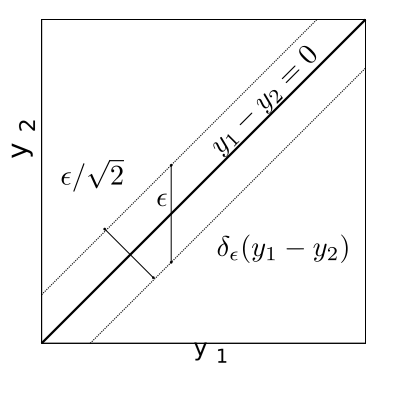
\includegraphics[width=0.5\textwidth]{FigurasPerfectas/DiagramaDelta01.pdf}
\caption{The surface $y_1=y_2$ and the approximation to its measure by
  $\epsilon$-width characteristic functions. Using the original coordinates
  we perform an error of $\sqrt{2}$, but using the $y,Y$ coordinates
  we arrive to the correct expresion. Using the MonteCarlo Numerics, this
  error is dificult to detect, because both the numeric and the wrongly solved
  analityc formula have the same multiplicative mistake. Is only when we plug this into
Machta Zwanzig Formula that the error becomes evident. }\label{DiagramaDelta01}
\end{figure}

The simplest approach to this integral is using directly the expression in the $y$ and $Y$
coordinates, since the surface is orthogonal to the $Y$ axis:
  \begin{align}
    A_\text{hopp}/8 & = \int_0^{a\sqrt{2}} \rd x  \int_{-b\sqrt{2}}^{b \sqrt{2}} \rd y
    \int_0^{a\sqrt{2}-x} \rd X  \int_0^{b \sqrt{2}-y} \rd Y
    \indicator{x^2+y^2 \geq 2 r^2} \delta (y) \label{pasoraro} \\
    &=  \int_0^{a\sqrt{2}} \rd x  \int_{-b\sqrt{2}}^{b \sqrt{2}} \rd y
    (a\sqrt{2}-x)(b\sqrt{2}-y)
    \indicator{x^2+y^2 \geq 2 r^2} \delta (y)\\
    &= \int_0^{a\sqrt{2}} \rd x b\sqrt{2} (a\sqrt{2}-x)
    \indicator{x^2\geq 2 r^2} \\
    &= \int_{r\sqrt{2}}^{a\sqrt{2}} \rd x
    (2ab-xb\sqrt{2})\\
    &=\biggl[2abx-\frac{x^2b}{\sqrt{2}} \biggr]_{r\sqrt{2}}^{a\sqrt{2}}\\
      A_\text{hopp}&=8\sqrt{2}b(a-r)^2
  \end{align}
  Note that in \eqref{pasoraro} we do not use symmetry in
  $y$, due to the Dirac delta.
  Here we have to apply the reasoning that was outlined in section \ref{knownfacts}.
  Given that this event can be realized in two ways which are
  distinguishable by their direction, it is as if the surface has two sides.
  Thus, we can incorporate a multiplicative factor of $s=2$ into this expression, or include it in the denominator of 
  the expression for the mean time.

  \subsubsection{Disc collisions}
  For other cross-section areas we proceed in a similar manner. 
  Disc collisions occur when $\sqrt{x^2 + y^2} = r \, \sqrt{2}$, giving
  \begin{align}
    A_\text{col}/16 & =\int_{x=0}^{a\sqrt{2}} \int_{X=0}^{a\sqrt{2}-x} \int_{y=0}^{b\sqrt{2}} \int_{Y=0}^{b\sqrt{2}-y}
    \rd x \rd X \rd y \rd Y
    \delta (\sqrt{x^2+y^2}-\sqrt{2}r)\\
    A_\text{col}/16 & =\iint _{0,0}^{a\sqrt{2},b\sqrt{2}}
    \rd x \rd y 
   \bigl[ 2ab-\sqrt{2}(ay+bx)+xy \bigr]
    \delta (\sqrt{x^2+y^2}-\sqrt{2}r)\\
    \end{align}
  We change to polar coordinates as we did in \ref{VolApen}:
  \begin{align}
    x^2+y^2 =: \rho \\   \Rightarrow   \delta(\sqrt{x^2+y^2}-\sqrt{2}r) \rightarrow
    \delta(\rho-\sqrt{2}r)   
    \end{align}
  Then we continue straightforwardly:
    \begin{align}
    A_\text{col}/16 & =\iint 
    \rd \theta \rd \rho \rho
    \bigl[2ab-\sqrt{2}\rho(a\sin\theta+b\cos\theta)+\rho^2\cos\theta\sin\theta
      \bigr]
    \delta(\rho-\sqrt{2}r) \\
    &=\int_\beta^\alpha \rd \theta \sqrt{2}r
    \bigl[
      2ab-2r(a\sin\theta+b\cos\theta)+2r^2\cos\theta\sin\theta)
      \bigr] \\
    A_\text{col} & = 16\sqrt{2} \bigl( 2abr(\alpha-\beta)
    + 2r^2 [a (\cos \alpha-\cos\beta) -b (\sin\alpha -\sin\beta)]
     + r^3(\sin^2 \alpha -\sin^2\beta) \bigr)
    \end{align}
    We have used the same trick as in previous subsection to obtain a general expression
    that works even when hopping is not possible. In the case of $r<w/4$ (all hopping possible)
    we have the substitution $\alpha=\pi/2$ and $b=0$, obtaining the result stated previously
    in eq. \ref{AreaChoque}. It is practical to leave here the expression for 1/4 of the
    total area. The symmetry of the cases makes it so that when the phase space splits
    into disjoint components, the volume accessible and the area accessible scale in
    the same manner.
    
    \subsubsection{Wall collisions}

    For a collision with the wall, the $x_i$ give suitable coordinates. Once again, we
    have to be careful with the multiplicative factors that appear due to change
    of variables. Let us suppose that we want the area that represents hits of
    the disc 2 against the right wall. That means that $x_2-a=0$. 
    \begin{align}
      A_{x_2=a} & =\iiiint_{-a,-a,-b,-b}^{a,a,b,b} \rd x_1 \rd x_2 \rd y_1 \rd y_2 
      \indicator{(x_1-x_2)^2+(y_1-y_2)^2 \geq (2 r)^2} \delta (x_2-a)\\
      &=\iiint_{-a,-b,-b}^{a,b,b} \rd x_1  \rd y_1 \rd y_2 
      \indicator{(x_1-a)^2+(y_1-y_2)^2 \geq (2 r)^2} 
    \end{align}
    Changing variables;
    \begin{equation}
      \frac{y_1-y_y}{\sqrt{2}} =  y  \qquad \frac{y_1+y_y}{\sqrt{2}}=Y \qquad \frac{x_1-a}{\sqrt{2}}=x
    \end{equation}
    Integrating over $x$,
    \begin{align}\label{areachoquexy}
      A_{x_2=a} & =\sqrt{2}\iiint_{-\sqrt{2}a,-\sqrt{2}b,-\sqrt{2}b+|y]}^{0,\sqrt{2}b,\sqrt{2}b-|y|}
        \rd x \rd y \rd Y 
      \indicator{(x^2+y^2 \geq 2 r^2} \\
      &=2\sqrt{2}\iint_{-\sqrt{2}a,-\sqrt{2}b}^{0,\sqrt{2}b}
        \rd x \rd y (\sqrt{2} b - |y|)
      \indicator{(x^2+y^2 \geq 2 r^2}
    \end{align}
    
    
    In the case that all hopping is possible there are no problems with the above derivations,
    but if vertical hopping is excluded, then there are differences.
    We must acknowledge some impossibles. If $r>h/4$, and the disc 2 starts
    on the left, it will never be able to hit the right wall. So, actually, this
    is a subsystem of the whole dynamic system in which our general formula needs
    to be adjusted. We can trace this problem to the original purpose of
    formula \ref{meanfreetime}
    was to find mean escape times. A particle cannot escape a volume if the exit is
    not in contact with that volume. So after hopping in one or both direction
    becomes impossible, the dynamical system gets split into disjoint components
    that never mix under the dynamics (ergodic components). So we have to take that
    into account. When $h/4<r<w/4$, a disk cannot interchange left-right positions,
    but can still move across all vertical available space.  After $r\geq w/4$,
    the system gets split again into two more disjoint components.
    So, when we calculate the ``avaible'' volume, we shall only use the
    part of the volume that belongs to the specific set that has a possibility of
    generating an event. We shall take into account what is written in the last
    paragraphs of the previous subsection. In this particular case, it is
    if as the volume gets split into disjoint components, namely 1,2 or 4 of the
    total avaible. This can be seen in the numerics as a discontinuity both
    in  the simulated data and in the exact expression. The avaible area
    for this event remains the same. 
    
    Again, it is simpler to evaluate the last expression in eq. \ref{areachoquexy}
    in the excluded space and then to subtract that from the whole configuration
    space evaluation.

    \begin{align}
      A_{x_2=a} & =4\sqrt{2}\iint_{0,0}^{\sqrt{2}a,\sqrt{2}b}
        \rd x \rd y (\sqrt{2} b - y)
        \indicator{(x^2+y^2) \geq 2 r^2}\\
     &=\underbrace{4\sqrt{2}\iint_{0,0}^{\sqrt{2}a,\sqrt{2}b}
        \rd x \rd y (\sqrt{2} b - y)}_{\text{whole space}}
        -\underbrace{
          4\sqrt{2}\iint_{0,0}^{\sqrt{2}a,\sqrt{2}b}
        \rd x \rd y \rd Y 
        \indicator{(x^2+y^2) < 2 r^2}(\sqrt{2} b - y)}_{\text{excluded space}}
       \end{align}
    The integrals are again routine to evaluate: the whole space part
    gives:
    \begin{equation}
      A_{\text{whole}}/4=8ab^2
    \end{equation}
    For the excluded part, we perform the same routine of evaluating the circular part
    in polar coordinates, and the triangular parts if they exist, in Cartesian.
    From the circular sector we get (see fig \ref{CasosIntegra} and the following explanation
    for $\alpha, \beta$ variables):
    \begin{equation}
      A_{sector}=8 b r^2(\alpha-\beta)+16r^3/3(\cos\alpha - \cos\beta)
    \end{equation}
    The upper triangle where to give, for $\alpha < \pi/2$,
    \begin{equation}
    A_{ut}=\frac{8}{3}b^2\sqrt{r^2-b^2}
    \end{equation}
    And the lower triangle a similar expression with $a$ instead of $b$.

    Now, this are actually all the expressions needed for any collision, but
    to combine them and to use them meaningfully is still needed. For example,
    this last calculated area could be used as representation of the event of
    the disc 1 hitting the right wall, or the disc 2 hitting the left wall. Both
    can make sense in the case of excluded horizontal interchange. What would be
    the expression of any disk hitting the right wall? It would be twice this expression
    but only before the exclusion sets in. Then we need to take into account
    the disjointedness of the phase space and divide the cases accordingly.

    In the same vein we could conclude that the area that represents
    any collision (wall, discs, etc) can be obtained by summing all the other
    areas, before hopping is excluded. If there is some sort of hindrance to
    the movement, then the expression becomes different, again, a sum over
    disjoint components. This could lead to tedious exercises in cases ramifications.

    
    
    

    

    
\section*{Acknowledgements}


DPS thanks Sidney Redner for asking the question that led to this work. Financial support is acknowledged from grants CONACYT-Mexico CB-101246 and CB-101997, and DGAPA-UNAM PAPIIT IN117117.





\bibliography{../../notasmixtas/TwoDiskBiblio}



\end{document}
